%%%%%%%% ICML 2018 EXAMPLE LATEX SUBMISSION FILE %%%%%%%%%%%%%%%%%

\documentclass{article}

% Recommended, but optional, packages for figures and better typesetting:
\usepackage{microtype}
\usepackage{graphicx}
\usepackage{subfigure}
\usepackage{booktabs} % for professional tables

% hyperref makes hyperlinks in the resulting PDF.
% If your build breaks (sometimes temporarily if a hyperlink spans a page)
% please comment out the following usepackage line and replace
% \usepackage{icml2018} with \usepackage[nohyperref]{icml2018} above.
\usepackage{hyperref}

% Attempt to make hyperref and algorithmic work together better:
\newcommand{\theHalgorithm}{\arabic{algorithm}}

% Use the following line for the initial blind version submitted for review:
% \usepackage{icml2018}

% If accepted, instead use the following line for the camera-ready submission:
\usepackage[accepted]{icml2018}

% The \icmltitle you define below is probably too long as a header.
% Therefore, a short form for the running title is supplied here:
\icmltitlerunning{Project Report for CS234 (Winter 2019)}

\usepackage{amsmath, amsthm, amssymb}

\graphicspath{{img/}} % set of paths to search for images

\newcommand{\bvec}[1]{\boldsymbol{#1}}
\newcommand{\dbvec}[1]{\dot{\boldsymbol{#1}}}
\newcommand{\ddbvec}[1]{\ddot{\boldsymbol{#1}}}
\DeclareMathOperator*{\argmin}{arg\,min}
\DeclareMathOperator*{\argmax}{arg\,max}


\begin{document}

\twocolumn[
\icmltitle{Project Report for CS234 (Winter 2019) \\
			Generalizing Locomotion Controllers}

% in order of appearance and this is the preferred way.
\icmlsetsymbol{equal}{*}

\begin{icmlauthorlist}
\icmlauthor{Li Quan Khoo}{stanford,scpd}
\end{icmlauthorlist}

\icmlaffiliation{stanford}{Computer Science Department}
\icmlaffiliation{scpd}{Stanford Center for Professional Development}

\icmlcorrespondingauthor{Li Quan Khoo}{lqkhoo@stanford.edu, li.khoo.11@ucl.ac.uk}

% You may provide any keywords that you
% find helpful for describing your paper; these are used to populate
% the "keywords" metadata in the PDF but will not be shown in the document
\icmlkeywords{Machine Learning, ICML}

\vskip 0.3in
] % \twocolumn

% this must go after the closing bracket ] following \twocolumn[ ...

% This command actually creates the footnote in the first column
% listing the affiliations and the copyright notice.
% The command takes one argument, which is text to display at the start of the footnote.
% The \icmlEqualContribution command is standard text for equal contribution.
% Remove it (just {}) if you do not need this facility.

\printAffiliationsAndNotice{}  % leave blank if no need to mention equal contribution
% \printAffiliationsAndNotice{\icmlEqualContribution} % otherwise use the standard text.

\section{Abstract}
Within the context of locomotion, given an agent, and a set of controllers for performing specific tasks (e.g. keep walking forward, keep walking sideways), is there a way to train a generalized policy that could perform all such tasks and also everything in between within the task-space (e.g. walk to any given point on the x-y plane)? In this report, we explore the method that inspired this work, the relation of this work to related concepts such as meta-learning, as well as our own attempt at solving this problem, in order to satisfy the given time constraints for this project.


\section{Introduction}
\subsection{Motivation}
In \cite{heess2017emergence} [\href{https://www.youtube.com/watch?v=hx_bgoTF7bs}{video}], using only simple reward functions, emergent locomotion behaviour was synthesized for humanoid models. The result is certainly impressive in that such behaviour could be trained even without the algorithm understanding the dynamics model.

However, since we are giving up so much information, we also notice quite immediately that several things could be improved. In particular, we immediately notice that is a certain unnaturalness or inefficiency of gait due to loose constraints (e.g. flailing arms in a running humanoid), jerkiness of motion due to discontinuous policy or feedback, in continuous state and action spaces. Training the policy can also be highly sample-inefficient due to lack of domain knowledge; it took Heess et. al. 6400 CPU-hours for their agent to learn this behaviour.

In our original proposal, the idea was to combine more specialized algorithms for learning the movements needed to solve particular tasks, and then leveraging this information to train a controller that could hopefully solve all such tasks, as well as any combination of them. When searching for prior work, it turned out quite quickly that this idea is hardly new. We based most of our initial ideas on two particularly interesting papers from Mordatch et. al., which we lightly explored in the project milestone:

\begin{itemize}
	\item Interactive Control of Diverse Complex Characters with Neural Networks \cite{mordatch2015interactive} [\href{https://www.youtube.com/watch?v=57D-qgVX-6o}{video}]
	\item Discovery of Complex Behaviors through Contact-Invariant Optimization \cite{mordatch2012discovery} [\href{https://www.youtube.com/watch?v=mhr_jtQrhVA}{video}]
\end{itemize}

\subsection{Background: Control Theory}

In the scope of rigid bodies interacting with the environment, locomotion can only happen via surface-to-surface contacts between the agent and the environment. These are temporary degrees of constraints (DOCs) depending on the nature of the contact (e.g. sliding, rolling, fixed), which are otherwise identical to joint articulations between rigid bodies. Although MuJoCo provides a highly simplified model of Newtonian fluids, for the sake of brevity, let's set aside fluid interactions for now.

This family of problems lies soundly in the field of control theory, which is about the study of the control of dynamical systems in continuous state spaces. As a simple example of a control system, consider a widely-used linear feedback control system, called the PID (proportional-integral-derivative) controller, whose control vector (the output, also called the response) $\bvec{u}$ is defined as:
\begin{align*}
\bvec{u}(t) &= w_1 \bvec{q}(t) + w_2\int_{t_1}^{t_2} \bvec{q}(t') dt' + w_3 \frac{d\bvec{q}}{dt}
\end{align*}

where $w$ terms are tunable scalar parameters, and $\bvec{q}$ is the state vector of the system, e.g. 6 the degrees of motion of a solid mass, or its temperature etc.

This could be understood as a controller whose response is linear with respect to the actual value of a variable, its instantaneous time delta, as well as moving average (whose job is to correct for a so-called steady-state error). It is notably not optimal for nonlinear systems.

More generally, in optimal control theory, we are interested in so-called "optimal" control, where the response of the controller satisfies some predefined optimality criterion, e.g. a minimum-time response.

\section{Related work}

\subsection{Model-Agnostic Meta-Learning (MAML)}
MAML, which was introduced in \cite{finn2017model}, is about learning a set of model parameters which make learning new (but related) tasks faster - quoting the paper directly - by finding \textit{model parameters that are sensitive to changes in the task, such that small changes in the parameters will produce large improvements on the loss function of any task}.

In contrast, and we are interested in generalizing to a wide range of motions, starting from a few specific tasks. For example, if we train the agent to walk forward one meter, we would like the agent to be able to generalize to walk forward any arbitrary distance. However, given a few tasks to begin with, depending on how the agent is trained, MAML could be useful to speed up the training process, although this is not directly applicable to Mordatch et. al.'s approach, which we shall cover later, because they use trajectory optimization to learn optimal policies for individual tasks.

\subsection{Mordatch et. al. 2015}
In Interactive Control of Diverse Complex Characters \cite{mordatch2015interactive}, the authors first trained their agent on individual tasks using trajectory optimization, and then proceeded to generalize their policy to the point where the agent can fly to any indicated point as indicated by the cursor. This is the main paper we studied, and is the main reason behind the work leadning up to this report. The authors put emphasis on a few important concepts as follows:

\subsubsection{Additive noise}
In \cite{mordatch2015interactive}, citing other prior work, states that injecting noise during training makes the resulting policy more robust, and noise is added to prevent divergent policies during execution. They add independent Gaussian noise $\epsilon \sim \mathcal{N}(\bvec{0}, \bvec{\sigma}^2_{\epsilon}\bvec{I})$ to all sensory inputs, and showed that if the noise is small enough, the optimal action at nearby noisy states is given by the first-order Taylor approximation $\bvec{a}(\bvec{s}+\epsilon) \approx \bvec{a}(s) + \frac{d\bvec{a}}{d\bvec{s}}\epsilon$.

Similarly, they added Gaussian noise $\gamma \sim \mathcal{N}(\bvec{0}, \bvec{\sigma}^2_{\gamma}\bvec{I})$ to the outputs of their hidden layers, as a network regularizer, in order to make the controller less sensitive to specific values of the hidden units.

The authors emphasized (and showed) the importance of this noise in the robustness of their resulting policies.

\subsubsection{Contact-Invariant Optimization (CIO)}
This is the main idea behind the 2012 paper. CIO optimizes over a composite objective function which is linear across four different loss terms. As defined in \cite{mordatch2012contact}:

\begin{align*}
L(\bvec{s}) &= L_{CI}(\bvec{s}) + L_{Physics}(\bvec{s}) + L_{Task}(\bvec{s}) + L_{Hint}(\bvec{s})
\end{align*}

For brevity, we shall not reproduce all the equations for individual losses here; please refer to the original paper for details. The important things are: all component losses are defined as $L_2$ losses, and all constraints, including contact points, are defined as soft, continuous functions, to enable numerical optimization. $L_{Hint}$ is an optional initialization heuristic, and it's defined as the zero-moment point (ZMP) stability criterion, to keep the ZMP in the convex hull of support regions. $L_{Task}$ encompasses losses over final poses, as well as energy efficiency and acceleration. $L_{Physics}$ enforces soft joint constraints and mesh collisions.

In order to specify the contact-invariant loss $L_{CI}$, the authors specified end-effector surfaces, which are the only surfaces allowed to exert forces on the environment. Each end-effector has an associated scalar variable $c_i$ that represents the contact force which the effector is exerting on the contact surface (e.g. in order to walk, push, grab etc.).

\begin{align*}
	L_{CI}(\bvec{s}) = \sum_{t}^{T}c_{i,t}(\bvec{s}) (||\bvec{e}_{i,t}(\bvec{s})||^2 + ||\dbvec{e}_{i,t}(\bvec{s})||^2 )
\end{align*}

where $\bvec{e}$ is a 4D $(x,y,z,\theta)$ contact-violation vector, and $\dbvec{e}$ the slippage penalty term.

There are variants of the loss function, especially in the $L_{CI}$ term to account for non-planar contacts \cite{mordatch2012contact}, but the most important feature of this loss is its decomposability. By disabling or enabling different components at different times, it can speed up the process of trajectory search. In the oral session, the authors start only with task and hint losses (thus ignoring all physical constraints and collisions) to generate an overly-optimistic solution, and then gradually re-enable other loss terms to converge onto a plausible solution trajectory.

\section{Approach}

\subsection{Approach 1: Block-alternate training with trajectory optimization}

\begin{algorithm}[tb]
	\caption{Block-alternate training with TO}
	\begin{algorithmic}
		\STATE Let policies be parameterized by $\theta$ and $\theta_i$ respectively
		\STATE Initialize policies $\pi$ and $\pi_i \forall i$ randomly
		\FOR{$N$ optimization cycles}
			\STATE Let $r_i$ be the reward of each individual task
			\FOR{each task $i$}
				\STATE Sample $\{s,a,r\}_i$ from environment by trajectory optimization
				\STATE $\pi_i \leftarrow \argmax_{\theta_i} \sum_{t}^{T} (\gamma^{T-t}r_i - ||a_\pi - a_i||^2) $
			\ENDFOR
			\STATE $\pi \leftarrow \argmin_{\theta} \sum_{i} ||a_\pi - a_i||^2$
		\ENDFOR
	\end{algorithmic}
\end{algorithm}

Our original intention was to follow Mordatch et. al.'s method and simplify as necessary, as proposed in the milestone.

We followed the plan and started implementing the piepline, while attempting to understand enough about trajectory optimization in order to implement the problem, but about a week before the deadline, it became quite clear that this wasn't going to happen. We had to come up with an alternative or we are not going to finish the project. Just to be clear, there are commercial and free libraries available for solving control problems, but first, they require formulating the objective in terms of an LQP (linear-quadratic problem) or similar.

\subsection{Appproach 2: Policy over policies}

\begin{algorithm}[tb]
	\caption{Policy over policies}
	\begin{algorithmic}
		\STATE Let policies be parameterized by $\theta$ and $\theta_i$ respectively
		\STATE Initialize policies $\pi$ and $\pi_i \forall i$ randomly
		\STATE Let $r_i$ be the reward of each individual task
		\FOR{each task $i$}
			\STATE Sample $\{s,a,r\}_i$ from environment by trajectory optimization
			\STATE $\pi_i \leftarrow \argmax_{\theta_i} \sum_{t}^{T} (\gamma^{T-t}r_i - ||a_\pi - a_i||^2) $
		\ENDFOR
		\STATE For generalized task, sample $\{s,a,r\}_i$ from environment
		\STATE $\pi \leftarrow \argmax_{\theta_i} \sum_{t}^{T} \gamma^{T-t}r $
	\end{algorithmic}
\end{algorithm}

Without sufficient knowledge to train an optimal controller for our agent, RL saves the day! What if we assumed that some policy trained using reinforcement learning was optimal for some individual task, and tried to work with that instead? The immediate benefit is that this removes our biggest roadblock and allows us to get at the central question behind this study, which is about generalizing from individual policies.

Perhaps the most immediate idea is to collect state-action pairs ${(s, a)}$ from running the individual task policies $\pi_i$ and attempt to fit a new policy $\pi$ by minimizing the error between $a$ and $a_\pi$, where $a_\pi$ is the set of actions of this new policy, by performing so-called policy regression. However, in the video presentation for \cite{mordatch2015interactive}, it was clear that this approach would not be correct. Quoting the example they gave, the agent's behaviour for individual tasks may be multimodal. Walking forward may start with the left foot, or the right foot, but taking the average action would not result in the agent walking forward.

Instead, we shall train a policy whose action space is limited to choosing which individual policy to follow, including the policy of doing nothing, in any given time step. One could think of this as making an ensemble out of the trained policies in order to best solve a composite task. We also had the idea of letting this policy scale the actions of individual policies by a scalar constant, but how much benefit this may confer to performance remains to be tested. Certain choices of this constant may also lower performance.

For instance, consider the task of leaping across a gap. Having the option to scale down the action parameters may cause the agent to simply fail more often. On the other hand, consider an agent trained to run either in the x or y direction at full speed. Suppose we want the agent to move to some arbitrary location on the x-y plane and then stop. Having the option to scale down the action may cause the agent to lose balance, depending on the model we are using, but on the other hand, avoids the issue of having to ping-pong between extreme policies when nearing or when overshooting the goal.

Training this is a straightforward two-part process: first we train individual task policies, then we train the generalized policy. Now conceptually, why might this be better than simply training the generalized policy directly? Suppose the composite task is highly complex e.g. swim, then leap across a gap, then walljump up to the goal. It may be much easier to train the agent on individual tasks first, before attempting to solve them all in sequence.

We could immediately identify several weaknesses about this method:
\begin{itemize}
	\item Its action space is linear in the number of individual tasks, so it may not scale well over multiple tasks.
	\item This method is computationally-inefficient, since during run-time, we still need to evaluate the individual task policies for the general policy to choose from.
\end{itemize}

\subsection{Approach 3: Block-alternate optimization revisited}

\begin{algorithm}[tb]
	\caption{Block-alternate training with RL}
	\begin{algorithmic}
		\STATE Let policies be parameterized by $\theta$ and $\theta_i$ respectively
		\STATE Initialize policies $\pi$ and $\pi_i \forall i$ randomly
		\FOR{$N$ optimization cycles}
			\STATE Let $r_i$ be the reward of each individual task
			\FOR{each task $i$}
				\STATE Sample $\{s,a,r\}_i$ from environment by MC policy rollout under $\pi_i$
				\STATE $\pi_i \leftarrow \argmax_{\theta_i} \sum_{t}^{T} (\gamma^{T-t}r_i - ||a_\pi - a_i||^2) $
			\ENDFOR
			\STATE $\pi \leftarrow \argmin_{\theta} \sum_{i} ||a_\pi - a_i||^2$
		\ENDFOR
	\end{algorithmic}
\end{algorithm}

Due to lack of time, primarily due to how many optimizing cycles we have to retrain the policies for each individual task, we have to leave this part as future work:

Let $\pi$ be the generalized policy and $\pi_i$ be individual task policies $\pi_i$. In each optimization cycle, we first train policies for solving individual tasks, maximizing discounted reward, but also penalizing for deviations in action space from the action output by the generalized policy. After this we simply perform policy regression on $\pi$ to update the generalized policy.

This is approach just swaps the trajectory-optimization step in the first approach with black-box optimization. The issue is that it would potentially take much longer for the algorithm to converge onto the general policy due to high variance of the proposed trajectories.

\section{Method}
\begin{figure}[H]
	\centering
	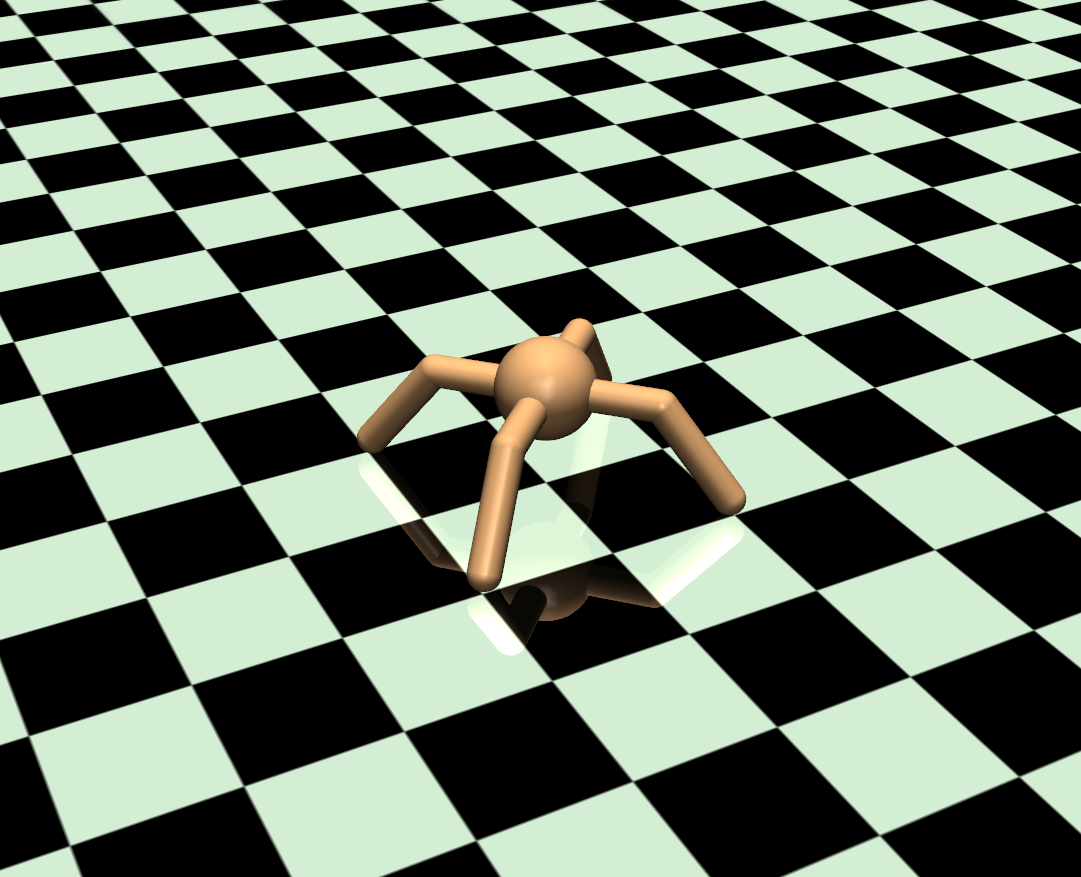
\includegraphics[width=0.9\linewidth]{ant_agent.png}
	\caption{The Ant model}
\end{figure}
For our choice of agent, we decided to use a standarized model, so that we may be able to make use of baseline results (if any). We decided on the Ant model, which is the simplest model available from the \texttt{gym} library which is also not constrained to moving along the x-z plane. The ant model has an eight-dimensional continuous action space, having 4 hip actuators that move the legs forwards and backwards relative to the torso, and 4 ankle actuators that move the legs inwards and outwards. It is also physically stable model with a low center of gravity, and isn't prone to toppling over, even under a zero-actuation policy, unlike the humanoid models. Since it has 4 legs, it isn't neccessary for the agent to learn how to balance in order to move properly, unlike the hopper model.

We trained the individual task policies using REINFORCE with normalized advantage, since the method and architecture worked very well for halfcheetah in Assignment 3. Both the policy and the baseline are implemented as dense feedforward networks in Tensorflow \cite{abadi2016tensorflow} with 3 hidden layers of 32 hidden units each, with ReLU activations, feeding into the final affine layer without any activations.

As of time of writing, we are working on the generalized policy network, with one discrete output for choosing the active policy, and a continuous output, for scaling the output of the active policy. It is important to note that it is not sufficient to simply scale the output to negative in order to run a policy in reverse, since the relationship between the action of each actuator and the resulting movement is highly nonlinear: consider the case where the leg has reached the end of its actuation range and needs to be reset. Running the policy in reverse would simply make the leg get stuck.

\section{Results}
Training on the modified OpenAI gym Ant-v3 environments for each individual task takes about 3 hours of computation time to complete 100 iterations of policy gradient, using the parameters we specified.

\begin{figure}[H]
	\centering
	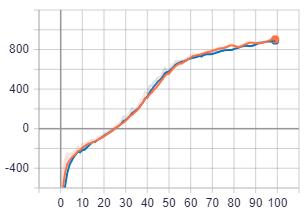
\includegraphics[width=0.9\linewidth]{antxy_avg_reward.png}
	\caption{Average reward for modified Ant-v3, tasked with running in positive x and y as fast as possible.}
\end{figure}

We are currently training the policies for running in negative x and y, with all remaining results pending. With some luck, we hope to have more to share before the poster presentation.

\section{Conclusion}
At this stage, unfortunately there is little we can conclude about our method, since we are still in the process of evaluating it. While our computer crunches away at training the policies, let's conclude our approach to the problem, and what we've learned from the process instead.

\subsection{General}
\begin{itemize}
	
	\item In the project milestone, we acknowledged the novelty of the problem domain with respect to our skillset, and consequently the difficulty of scoping the project in order to meet the hard deadline. In response, we defined our goals as a priority list in order to mitigate this problem. However, that list was defined based on the assumption that we would work along the lines of Mordatch et. al.'s approach. Without a better understanding of trajectory optimization ahead of time, however, it is not clear whether we could have done any better defining the goal list.
	
	\item Many of the tools necessary for the project were unfamiliar to us. This includes MuJoCo itself, its Python wrappers dm\_control and mujoco-py (which are incompatible with each other). We accounted for this when budgeting for time, but there are many things which we did not manage to forsee. For example, we still do not know how to properly initialize an \texttt{mjvperturb} instance in order to move the model, but we had to drop such tasks or work around limitations of the given Viewers because we simply lack the time to investigate further.
	
\end{itemize}
\subsection{Frameworks}
\begin{itemize}
	
	\item Setting up the environment such that entire pipeline works was not a trivial process that took a number of days, and it involved a lot of trial and error and searching forums about the relevant errors. We have fully documented the steps we took to set up the environment both in the cloud and locally (on a Windows machine) in the documentation (repo link in appendix).
	
	\item As far as we are aware of, there are no tutorials for MuJoCo \cite{todorov2012mujoco} available. We took quite some time starting from understanding the basics like what the difference is between a body and a geom, up to how to prevent collisions between the agent and the goal target geom (via setting the \texttt{conaffinity} properties), about half the time by changing the XML model specification and observing the changes through trial and error. Working with the actual values like the quarternions also requires some working knowledge of kinematics. Depending on how involved the task at hand is, one might even need to make some OpenGL function calls in order to get the required data from the scene, such as when we needed to implement the ray-tracer.
	
	\item Deepmind control suite (dm\_control) \cite{tassa2018deepmind} came prepackaged with a Viewer class that provides a view into the scene of the agent and the environment, that supports perturbation forces (push / pull / rotate the model) out of the box. As of March 2019, we found it very difficult to add and configure our own environments. As a workaround, we installed dm\_control as a Python module, but we also included the full source as a submodule in our source code, so we could add in the environments as needed, by importing them from source. We found dm\_control less easy to 'hack' around in. For instance, the Viewer depends on having a fully-defined environment to work. The source code doesn't appear to have versioning, i.e. \texttt{pip show dm\_control} always returns version 0.0.0, so it's difficult to say whether this will persist in the future.
	
	\item mujoco-py is OpenAI's wrapper for MuJoCo. In certain ways it is less sophisticated than dm\_control, but sometimes that's a good thing. For example, the Viewer does not directly support force perturbation, and we had to manually implement a ray-tracer in order to point to scene coordinates, in order to move the goal target. However, what we liked about the wrapper is that the important properties in the simulator and data objects mirror MuJoCo's API, which makes referencing MuJoCo's comprehensive native documentation much more straightforward, since the documentation of both of these wrappers are lacking. In contrast, dm\_control uses an Indexer class to re-assign properties to each geom or body, which can make locating a particular value a chore, especially if we are interested in, say, the positions of a subset of geoms or bodies, rather than just a single one.
\end{itemize}

\section{Future Work}
It would be nice to follow through with Approach 3, but it's probably a better idea to take the necessary time to study trajectory optimization sufficiently to implement the original idea as proposed.

\section{Acknowledgements}
I would like to thank the entire CS234 teaching staff. Without their assistance, this work - limited as it is - would not have been possible.

\section{Appendix}
For source code, please refer to the repository: \href{https://github.com/lqkhoo/cs234-winter-2019}{https://github.com/lqkhoo/cs234-winter-2019}

\newpage

\bibliography{report}
\bibliographystyle{icml2018}


%%%%%%%%%%%%%%%%%%%%%%%%%%%%%%%%%%%%%%%%%%%%%%%%%%%%%%%%%%%%%%%%%%%%%%%%%%%%%%%
%%%%%%%%%%%%%%%%%%%%%%%%%%%%%%%%%%%%%%%%%%%%%%%%%%%%%%%%%%%%%%%%%%%%%%%%%%%%%%%
% DELETE THIS PART. DO NOT PLACE CONTENT AFTER THE REFERENCES!
%%%%%%%%%%%%%%%%%%%%%%%%%%%%%%%%%%%%%%%%%%%%%%%%%%%%%%%%%%%%%%%%%%%%%%%%%%%%%%%
%%%%%%%%%%%%%%%%%%%%%%%%%%%%%%%%%%%%%%%%%%%%%%%%%%%%%%%%%%%%%%%%%%%%%%%%%%%%%%%

\end{document}


% This document was modified from the file originally made available by
% Pat Langley and Andrea Danyluk for ICML-2K. This version was created
% by Iain Murray in 2018. It was modified from a version from Dan Roy in
% 2017, which was based on a version from Lise Getoor and Tobias
% Scheffer, which was slightly modified from the 2010 version by
% Thorsten Joachims & Johannes Fuernkranz, slightly modified from the
% 2009 version by Kiri Wagstaff and Sam Roweis's 2008 version, which is
% slightly modified from Prasad Tadepalli's 2007 version which is a
% lightly changed version of the previous year's version by Andrew
% Moore, which was in turn edited from those of Kristian Kersting and
% Codrina Lauth. Alex Smola contributed to the algorithmic style files.
